\section{Hyperbolic thermal explosion: exponential nonlinearities}
\label{therm:sec}

In fast thermal processes (pulsed laser heating and processing, ignition of
solid propellants and energetic materials, rapid combustion) the relevant time
scales can approach the thermal relaxation time of the medium, and Fourier's law
is replaced by the Maxwell--Cattaneo--Vernotte (MCV) law
\cite{Cattaneo1958,Vernotte1958,JosephPreziosi1989,Straughan2011}.  Combined
with the Frank-Kamenetskii (FK) exothermic source
\cite{FrankKamenetskii1955,BebernesEberly1989}, this produces damped wave
equations with exponential nonlinearities.  The main points of this section are:
\begin{enumerate}[label=(\arabic*),leftmargin=2em]
\item There are two inequivalent hyperbolic models (``reduced'' and ``full'');
  their blowup is \emph{qualitatively different}.
\item Reduced model: the ODE blowup $\theta\simeq\log(2\tau_*/\delta)-2\log(T-t)$ is
  stable modulo time translation and Lorentz boosts; the linearised spectrum is
  explicit, the spectral gap is $1$ (\cref{therm:thm:reduced}).
\item In $d=1$ the reduced model is Liouville's equation; the explicit general
  solution confirms the theorem, including the sharpness of the gap
  (\cref{therm:sec:liouville}).
\item Full (MCV-consistent) model: the blowup is $\theta\simeq-\log\bigl(\delta(T-t)\bigr)$ (the
  \emph{parabolic} rate) with a \emph{hyperbolic} spatial structure; there is no
  Lorentz invariance, the neutral modes come from a family of tilted plane
  waves, and $\lambda=-1$ carries a Jordan block (\cref{therm:sec:full}).
\item With Arrhenius kinetics there is no blowup at all; FK blowup is an
  intermediate asymptotic regime (\cref{therm:sec:arrhenius}).
\end{enumerate}
Throughout, \emph{known} results are attributed, statements labelled
``proof sketch'' are derived here with the Donninger machinery but not written
out in full detail, and purely numerical observations are labelled as such.
All algebraic identities below are verified symbolically in
\texttt{code/therm\_symbolic.py}; spectra in \texttt{code/therm\_spectrum.py};
simulations in \texttt{code/therm\_sim1d.py}.

% ---------------------------------------------------------------------------
\subsection{Modelling: Cattaneo flux and Frank-Kamenetskii source}
\label{therm:sec:model}

Let $\Theta$ be the absolute temperature, $\Theta_0$ the ambient temperature,
$\rho c$ the volumetric heat capacity, $k$ the conductivity, $\tau_r$ the thermal
relaxation time, and $Q A e^{-E/(R\Theta)}$ the volumetric heat release
(zeroth-order Arrhenius kinetics, reactant consumption neglected).  Energy
balance and MCV law read
\begin{equation}\label{therm:eq:phys}
  \rho c\,\partial_t\Theta+\nabla\!\cdot q=QA\,e^{-E/(R\Theta)},\qquad
  \tau_r\,\partial_t q+q=-k\nabla\Theta .
\end{equation}
With the FK variable $\theta=E(\Theta-\Theta_0)/(R\Theta_0^2)$ and
$\varepsilon=R\Theta_0/E$ one has the \emph{exact} identity
$e^{-E/(R\Theta)}=e^{-E/(R\Theta_0)}\exp\bigl(\theta/(1+\varepsilon\theta)\bigr)$.
Scaling $x=Lx'$, $t=t_0t'$ with the diffusion time $t_0=\rho cL^2/k$, and
$q=(kR\Theta_0^2/(EL))\,q'$, gives (primes dropped)
\begin{equation}\label{therm:eq:system}
  \theta_t+\nabla\!\cdot q=f_\varepsilon(\theta):=\delta\,e^{\theta/(1+\varepsilon\theta)},\qquad
  \tau_*\, q_t+q=-\nabla\theta,
\end{equation}
with the FK parameter $\delta=QAEL^2e^{-E/(R\Theta_0)}/(kR\Theta_0^2)$ and the
dimensionless relaxation time $\tau_*=\tau_r/t_0=\tau_rk/(\rho cL^2)$; the
dimensionless thermal wave speed is $\tau_*^{-1/2}$.  Applying $(1+\tau_*\partial_t)$ to
the balance law and subtracting the divergence of the flux law eliminates $q$:
\begin{equation}\label{therm:eq:full}
  \boxed{\ \tau_*\theta_{tt}+\theta_t-\Delta\theta=f_\varepsilon(\theta)+\tau_*\,\partial_t f_\varepsilon(\theta)
  =f_\varepsilon(\theta)+\tau_* f_\varepsilon'(\theta)\,\theta_t\ }\qquad\text{(full model)}.
\end{equation}
\Cref{therm:eq:full} with data $(\theta,\theta_t)|_{t=0}=(\theta_0,\theta_1)$ is
equivalent to \cref{therm:eq:system} with any $q_0$ satisfying
$-\nabla\cdot q_0=\theta_1-f_\varepsilon(\theta_0)$.  The \emph{reduced} model
\begin{equation}\label{therm:eq:reduced}
  \tau_*\theta_{tt}+\theta_t-\Delta\theta=f_\varepsilon(\theta)\qquad\text{(reduced model)}
\end{equation}
drops the term $\tau_*\partial_tf_\varepsilon(\theta)$.  It is obtained if the
relaxation is applied to the \emph{whole} energy balance (a single phase lag
$\rho c\,\Theta_t(t+\tau_r)=-\nabla\!\cdot q_{\rm Fourier}(t)+Q(t)$, expanded to first
order), or by discarding $\tau_*\partial_t f$ as small.  Both forms occur in the
literature on hyperbolic reaction--diffusion equations; e.g.\ the full form
$\tau_* n_{tt}+n_t=Dn_{xx}+F(n)+\tau_* F'(n)n_t$ is the starting point of
\cite{MendezFortFarjas1999}, while the reduced form is what one obtains by simply
adding $\tau_*\theta_{tt}$ to the parabolic Gelfand problem.  We could not
verify, within our (limited) literature search, which of the two forms is used
in the thermal-explosion-specific literature; the distinction is essential near
blowup.
% TODO verify: specific thermal-explosion/ignition papers with Cattaneo flux
% (search budget exhausted before these could be checked).
We show below that the dropped term is \emph{dominant} at blowup, so the two
models are not asymptotically equivalent near thermal runaway.

\paragraph{Normal forms.}  In the FK limit $\varepsilon\to0$, $f_0(\theta)=\delta e^\theta$.
Rescale time $t\mapsto\sqrt{\tau_*}\,t$ (wave speed $1$) and put $\gamma:=\tau_*^{-1/2}$.
The reduced model becomes (keeping $\delta$, as in the conventions)
\begin{equation}\label{therm:eq:redN}
  u_{tt}+\gamma u_t-\Delta u=\delta e^{u},\qquad u(t,x)=\theta(\sqrt{\tau_*}\,t,x),
\end{equation}
and the full model becomes, with $u(t,x)=\theta(\sqrt{\tau_*}\,t,x)+\log(\sqrt{\tau_*}\,\delta)$,
\begin{equation}\label{therm:eq:fullN}
  (\partial_t+\gamma)\bigl(u_t-e^{u}\bigr)=\Delta u
  \quad\Longleftrightarrow\quad
  u_{tt}-\Delta u=e^{u}u_t+\gamma\,(e^{u}-u_t).
\end{equation}
Both are invariant under $u\mapsto u(\mu t,\mu x)+\kappa\log\mu$ ($\kappa=2$ reduced,
$\kappa=1$ full) \emph{provided} $\gamma\mapsto\mu\gamma$.  Hence the damping enters only
through the dimensionless product $\gamma T$ ($T$ = blowup time); near the
singularity it is a perturbation of relative size $\gamma(T-t)\to0$.

\begin{remark}[Quenching form]\label{therm:rem:quench}
For readers used to MEMS models: $w=e^{-u/2}$ turns \cref{therm:eq:redN} with
$\gamma=0$ into the quenching problem
$w_{tt}-\Delta w=\bigl(w_t^2-|\nabla w|^2\bigr)/w-\delta/(2w)$, and the ODE blowup below
becomes the linear touchdown $w=\sqrt{\delta/2}\,(T-t)$.
\end{remark}

% ---------------------------------------------------------------------------
\subsection{Reduced model: ODE blowup, symmetries, similarity variables}
\label{therm:sec:reduced}

Let first $\gamma=0$: $u_{tt}-\Delta u=\delta e^u$.  The spatially homogeneous
solutions satisfy $u''=\delta e^u$; those that blow up are
$e^{u}=2a^2/(\delta\sinh^2(a(T-t)))$, $2/(\delta(T-t)^2)$, $2a^2/(\delta\sin^2(a(T-t)))$,
all of the form $u=u_T+O((T-t)^2)$ with the \emph{ODE blowup}
\begin{equation}\label{therm:eq:ode}
  u_T(t)=\log\frac{2}{\delta}-2\log(T-t).
\end{equation}
\paragraph{Symmetries.}  Time and space translations, rotations, the scaling
$u\mapsto u(\mu t,\mu x)+2\log\mu$, the shift $u\mapsto u+c_0$, $\delta\mapsto
\delta e^{-c_0}$ (so $\delta$ can be normalised on $\mathbb{R}^d$), and Lorentz boosts.
Boosting \cref{therm:eq:ode} and re-centring the singular hyperplane at $(T,0)$ gives
the family (checked symbolically for $d=3$)
\begin{equation}\label{therm:eq:boosted}
  u_{T,a}(t,x)=\log\frac{2}{\delta}-2\log\bigl(A_0(T-t)+a\cdot x\bigr),\qquad
  A_0=A_0(a)=\sqrt{1+|a|^2},\quad a\in\mathbb{R}^d ,
\end{equation}
singular on the spacelike hyperplane $t=T+a\cdot x/A_0$ (velocity $a/A_0$,
$|a/A_0|<1$).  Space translations and scalings map $u_{T,a}$ to $u_{T',a}$, so
$\{u_{T,a}\}$ is the full $(d+1)$-parameter symmetry orbit of the ODE blowup for a
fixed blowup point $x_0=0$.

\paragraph{Similarity variables.}  With the conventions of the note,
$\tau=\log T-\log(T-t)$, $\xi=x/(T-t)$, $\Lambda=\xi\cdot\nabla_\xi$,
$\psi_1=u+2\log(T-t)$, $\psi_2=(T-t)u_t$, \cref{therm:eq:redN} becomes
\begin{equation}\label{therm:eq:simred}
  \partial_\tau\psi_1=-\Lambda\psi_1+\psi_2-2,\qquad
  \partial_\tau\psi_2=\Delta\psi_1-\Lambda\psi_2-\psi_2+\delta e^{\psi_1}-\gamma T e^{-\tau}\psi_2 .
\end{equation}
The boosted ODE blowups are \emph{static} solutions (for $\gamma=0$):
\begin{equation}\label{therm:eq:Psia}
  \Psi_a(\xi)=\Bigl(\log\tfrac{2}{\delta}-2\log(A_0+a\cdot\xi),\ \tfrac{2A_0}{A_0+a\cdot\xi}\Bigr),
  \qquad \Psi_0=\bigl(\log\tfrac2\delta,\,2\bigr),
\end{equation}
smooth on $\overline{B^d}$ for every $a$.  Writing $\psi=\Psi_0+\varphi$,
\begin{equation}\label{therm:eq:linred}
\begin{gathered}
  \partial_\tau\varphi=\mathbf L\varphi+\mathbf N(\varphi)-\gamma Te^{-\tau}(0,2+\varphi_2),\\
  \mathbf L\varphi=\begin{pmatrix}-\Lambda\varphi_1+\varphi_2\\ \Delta\varphi_1-\Lambda\varphi_2-\varphi_2+2\varphi_1\end{pmatrix},\qquad
  \mathbf N(\varphi)=\begin{pmatrix}0\\ 2(e^{\varphi_1}-1-\varphi_1)\end{pmatrix},
\end{gathered}
\end{equation}
since $\delta e^{c}=2$ for $c=\log(2/\delta)$; thus $V_0=2$, $s=0$ in the notation
of the note.

\paragraph{Damped homogeneous blowup.}  For $\gamma>0$ the profile \cref{therm:eq:ode} is
not exact.  A formal Fuchsian expansion of $u''+\gamma u'=\delta e^u$ gives
\begin{equation}\label{therm:eq:damped}
  u(t)=u_T(t)+\gamma(T-t)+\tfrac23\gamma^2(T-t)^2\log(T-t)+b\,(T-t)^2+\dots ,
\end{equation}
with a free constant $b$: the damping produces an $e^{-\tau}$ correction in
similarity variables and a resonant logarithm at order $e^{-2\tau}$ (the
$(T-t)^2$ mode is the eigenvalue $-2$ below).

% ---------------------------------------------------------------------------
\subsection{Linearised operator and its spectrum}
\label{therm:sec:spectrum}

Let $\mathcal H^k:=H^k(B^d)\times H^{k-1}(B^d)$, $k\in\mathbb{N}$, $k>d/2$.  Write
$\mathbf L=\mathbf L_0+\mathbf L'$ with the free part
$\mathbf L_0\varphi=(-\Lambda\varphi_1+\varphi_2,\ \Delta\varphi_1-\Lambda\varphi_2-\varphi_2)$
and $\mathbf L'\varphi=(0,2\varphi_1)$, which is compact on $\mathcal H^k$ (Rellich).

\begin{lemma}[Free evolution]\label{therm:lem:free}
Let $\varphi$ be a smooth solution of $\partial_\tau\varphi=\mathbf L_0\varphi$ and
$E_k(\varphi)=\|D^k\varphi_1\|_{L^2(B^d)}^2+\|D^{k-1}\varphi_2\|_{L^2(B^d)}^2$, where $D^j$ is the
tensor of all $j$-th derivatives.  Then
$\frac{d}{d\tau}E_k\le-2\bigl(k-\tfrac d2\bigr)E_k$.  Consequently the semigroup
generated by $\mathbf L_0$ on $\mathcal H^k$ has essential growth bound
$\le-(k-\tfrac d2)$; since $\{\operatorname{Re}\lambda<\tfrac d2-k\}\subset\sigma_p(\mathbf L_0)$, the
free decay rate on $\mathcal H^k$ is exactly $k-\tfrac d2$.  (The finitely many eigenvalues of
$\mathbf L_0$ with $\operatorname{Re}\lambda>\frac d2-k$, e.g.\ $\lambda=0$ with eigenfunction $(1,0)$, live on a
finite-dimensional invariant space of polynomials.)
\end{lemma}

\begin{proof}
Differentiating, $\partial_\tau D^k\varphi_1=-(\Lambda+k)D^k\varphi_1+D^k\varphi_2$ and
$\partial_\tau D^{k-1}\varphi_2=\Delta D^{k-1}\varphi_1-(\Lambda+k)D^{k-1}\varphi_2$.  Use
$-(\Lambda f,f)=\tfrac d2\|f\|^2-\tfrac12\int_{\mathbb S^{d-1}}|f|^2$ and integrate the
cross term by parts: $(D^k\varphi_2,D^k\varphi_1)+(\Delta D^{k-1}\varphi_1,D^{k-1}\varphi_2)
=\int_{\mathbb S^{d-1}}\partial_rD^{k-1}\varphi_1\cdot D^{k-1}\varphi_2$.  Hence
\[
\tfrac12\tfrac{d}{d\tau}E_k=-(k-\tfrac d2)E_k-\tfrac12\!\int_{\mathbb S^{d-1}}\!\bigl(|D^k\varphi_1|^2+|D^{k-1}\varphi_2|^2
-2\,\partial_rD^{k-1}\varphi_1\cdot D^{k-1}\varphi_2\bigr)\le-(k-\tfrac d2)E_k,
\]
because $|\partial_rD^{k-1}\varphi_1|\le|D^k\varphi_1|$ on $|\xi|=1$.  The kernel of $E_k$ is
$Y=\mathcal P_{k-1}\times\mathcal P_{k-2}$ (polynomials), which is finite dimensional
and $\mathbf L_0$-invariant; on $\mathcal H^k/Y$ the seminorm $E_k^{1/2}$ is an
equivalent norm (Bramble--Hilbert), and the induced quotient semigroup decays
like $e^{-(k-d/2)\tau}$.  This gives the bound on the essential growth bound.
Conversely, for $\operatorname{Re}\lambda<\tfrac d2-k$ both Frobenius solutions at $|\xi|=1$
of the eigenvalue equation (see the proof of \cref{therm:prop:spec}) lie in
$H^k$, so every such $\lambda$ is an eigenvalue.
\end{proof}

In the power case the same energy structure (with top-order rate $s+k-\frac d2$)
underlies the semigroup theory of \cite{DonningerSchoerkhuber2017,Ostermann2024},
which works with suitable equivalent inner products; we have not checked that
those constructions carry over verbatim to $s=0$, but the quotient argument
above is all that is used below.  Since $\mathbf L'$ is compact,
$\sigma(\mathbf L)\cap\{\operatorname{Re}\lambda>\frac d2-k\}$ consists of isolated eigenvalues of finite
algebraic multiplicity.

\begin{proposition}[Point spectrum, reduced model]\label{therm:prop:spec}
Let $k>d/2$ and $\operatorname{Re}\lambda>\frac d2-k$.  Then $\lambda\in\sigma_p(\mathbf L)$ if and only if
\begin{equation}\label{therm:eq:eigs}
  \lambda\in\{1-\ell-2n\}\cup\{-2-\ell-2n\},\qquad \ell,n\in\mathbb{N}_0
  \quad(\ell\in\{0,1\}\text{ if }d=1).
\end{equation}
The eigenfunctions are $\varphi=(g,(\lambda+\Lambda)g)$ with
$g=|\xi|^\ell Y_\ell(\xi/|\xi|)\,{}_2F_1(\alpha,\beta;\ell+\frac d2;|\xi|^2)$, a polynomial,
where $\alpha=\frac{\lambda+\ell-1}{2}$, $\beta=\frac{\lambda+\ell+2}{2}$ and $Y_\ell$ is a
spherical harmonic of degree $\ell$.
\end{proposition}

\begin{proof}
Eliminating $\varphi_2=(\lambda+\Lambda)\varphi_1$ gives, for $g=\varphi_1$,
\begin{equation}\label{therm:eq:eigpde}
  (\delta_{ij}-\xi_i\xi_j)\partial_i\partial_jg-2(\lambda+1)\Lambda g-\bigl(\lambda(\lambda+1)-2\bigr)g=0
  \quad\text{in }B^d .
\end{equation}
The operator is elliptic in the open ball, so $g\in C^\infty(B^d)$, and the
projection of $g$ onto spherical harmonics of degree $\ell$ has the form
$|\xi|^\ell Y_\ell\,h(\rho)$, $\rho=|\xi|^2$, with $h$ smooth on $[0,1)$.  A direct
computation (verified for general $d,\ell$) turns \cref{therm:eq:eigpde} into
$4|\xi|^\ell Y_\ell$ times the hypergeometric equation
$\rho(1-\rho)h''+[c-(\alpha+\beta+1)\rho]h'-\alpha\beta h=0$ with $c=\ell+\frac d2$ and $\alpha,\beta$
as stated.  Regularity at $\rho=0$ selects $h={}_2F_1(\alpha,\beta;c;\rho)$.  At
$\rho=1$ the Frobenius exponents are $0$ and $c-\alpha-\beta=\frac{d-1}{2}-\lambda$; the
corresponding branch $(1-\rho)^{\frac{d-1}{2}-\lambda}$ (multiplied by $\log(1-\rho)$ in
the integer case) is \emph{not} in $H^k$ near $\rho=1$, because
$\frac{d-1}{2}-\operatorname{Re}\lambda<k-\frac12$.  By the connection formulae
\cite[\S15.8]{OlverEtAl2010}, the coefficient of this branch in
${}_2F_1(\alpha,\beta;c;\rho)$ is a non-vanishing multiple of $1/(\Gamma(\alpha)\Gamma(\beta))$ in
all three cases $c-\alpha-\beta\notin\mathbb{Z}$, $\in\mathbb{N}_0$ (logarithmic term), $\in-\mathbb{N}$
(pole-type leading term $\Gamma(\alpha+\beta-c)\Gamma(c)/(\Gamma(\alpha)\Gamma(\beta))$).  Hence
$\lambda$ is an eigenvalue iff $\alpha\in-\mathbb{N}_0$ or $\beta\in-\mathbb{N}_0$, i.e.\
\cref{therm:eq:eigs}, and then ${}_2F_1$ is a polynomial.  (For $d=1$ use the
even/odd decomposition, $\ell\in\{0,1\}$.)
\end{proof}

\begin{table}[t]
\centering
\begin{tabular}{@{}cllll@{}}
\toprule
$\lambda$ & sector & eigenfunction $g$ & mult. & origin \\
\midrule
$1$ & $\ell=0$ & $1$ & $1$ & time translation $\partial_T u_{T,0}$\\
$0$ & $\ell=1$ & $\xi_j$ & $d$ & boosts, $\partial_{a_j}\Psi_a|_{a=0}=-2(\xi_j,\xi_j)$\\
$-1$ & $\ell=0,2$ & $1-|\xi|^2/d$; harm.\ quadratics & $1+\dim\mathcal Y_2$ & curvature of blowup surface\\
$-2$ & $\ell=0,1,3$ & $1$; \dots & & energy of the ODE; \dots\\
\bottomrule
\end{tabular}
\caption{Leading eigenvalues of $\mathbf L$ (reduced model, $V_0=2$, $s=0$).  The
interpretation of $\lambda=-1$ follows from the exact $1$D solution, \cref{therm:prop:liouville}.}
\label{therm:tab:eigs}
\end{table}

\begin{lemma}[Semisimplicity]\label{therm:lem:semisimple}
The eigenvalues $\lambda=1$ and $\lambda=0$ of $\mathbf L$ on $\mathcal H^k$, $k>d/2$, are semisimple.
\end{lemma}

\begin{proof}
Let $P(\lambda)g:=(\Lambda+\lambda)(\Lambda+\lambda+1)g-\Delta g-2g$.  A Jordan chain $(\mathbf L-\lambda_0)w=\varphi_0$
with $\varphi_0=(g_0,(\lambda_0+\Lambda)g_0)$ forces $P(\lambda_0)w_1=-P'(\lambda_0)g_0=-(2\Lambda+2\lambda_0+1)g_0$.
For $(\lambda_0,\ell)\in\{(1,0),(0,1)\}$ we have $g_0=|\xi|^\ell Y_\ell$, $\alpha=0$,
$\beta=\frac32$, and $P'(\lambda_0)g_0=3g_0$; in the $\ell$-sector this becomes
$\rho(1-\rho)h''+(c-\frac52\rho)h'=\frac34$.  Since
$\frac{d}{d\rho}\bigl[\rho^c(1-\rho)^{\beta+1-c}h'\bigr]=\rho^{c-1}(1-\rho)^{\beta-c}\bigl[\rho(1-\rho)h''+(c-(\beta+1)\rho)h'\bigr]$,
regularity at $0$ gives
$\rho^c(1-\rho)^{\frac52-c}h'(\rho)=\frac34\int_0^\rho s^{c-1}(1-s)^{\frac32-c}\,ds$.
Write $q=\frac52-c$.  If $q>0$ the right side tends to $\frac34B(c,q)\ne0$, so
$h'\sim\frac34B(c,q)(1-\rho)^{-q}$; if $q=0$ it diverges like $-\frac34\log(1-\rho)$;
if $q<0$, $q\notin\mathbb{Z}$, it equals $\frac34B(c,q)+(1-\rho)^q\times$(analytic) by
analytic continuation in $q$, with $B(c,q)=\Gamma(c)\Gamma(q)/\Gamma(\frac52)\neq0$, so again
$h'\ni\frac34B(c,q)(1-\rho)^{-q}$; if $q\in-\mathbb{N}$ the integrand contains
$(1-s)^{-1}$ with coefficient $(-1)^{c-5/2}\binom{c-1}{c-5/2}\neq0$, producing
$(1-\rho)^{-q}\log(1-\rho)$ in $h'$.  In every case $h\ni(1-\rho)^{c-\frac32}$ (times
$\log(1-\rho)$ in the integer cases) with non-zero coefficient, which is not in
$H^k$ near $\rho=1$ since $c-\frac32=\frac{d-1}{2}-\lambda_0<k-\frac12$.
\end{proof}

\begin{corollary}[Spectral gap]\label{therm:cor:gap}
For $k>d/2$ set $\omega_0:=\min\{1,k-\frac d2\}$.  Then
$\sigma(\mathbf L)\cap\{\operatorname{Re}\lambda>-\omega_0\}=\{0,1\}$; $\lambda=1$ is simple with eigenfunction
$(1,1)$, $\lambda=0$ is semisimple of multiplicity $d$ with eigenfunctions
$(\xi_j,\xi_j)$.  With $\mathbf P$ the Riesz projection onto these $d+1$ modes,
$\|e^{\tau\mathbf L}(1-\mathbf P)\|\le C_\omega e^{-\omega\tau}$ for every $\omega<\omega_0$.  If $k\ge\frac d2+1$,
then $\omega_0=1$.
\end{corollary}

\begin{remark}[Boosted profiles; polynomial structure; numerics]\label{therm:rem:numspec}
(i) A mode $e^{\lambda\tau}g(\xi)$ corresponds to the solution
$v=(T-t)^{-\lambda}g(x/(T-t))$ of the linearised equation, homogeneous of degree
$-\lambda$ in $(t-T,x)$; Lorentz transformations fixing $(T,0)$ preserve the
backward cone, homogeneity and smoothness and conjugate the linearisations at
$u_{T,0}$ and $u_{T,a}$.  Hence $\mathbf L_a$ (linearisation at $\Psi_a$) has the same
point spectrum \cref{therm:eq:eigs}.
(ii) $\mathbf L$ maps $\mathcal P_N\times\mathcal P_N$ (polynomials in $\rho$ times
$|\xi|^\ell Y_\ell$) into itself and is block upper-triangular in the monomial
basis, with diagonal blocks $\begin{psmallmatrix}-(\ell+2m)&1\\2&-(\ell+2m)-1\end{psmallmatrix}$, whose
eigenvalues are exactly $1-\ell-2m$ and $-2-\ell-2m$ -- a two-line proof that
\cref{therm:eq:eigs} are eigenvalues (completeness needs the connection
argument).  Consequently Chebyshev collocation in $\rho$ is exact in exact
arithmetic; in floating point ($N=32$) it reproduces \cref{therm:eq:eigs} to within
$3\cdot10^{-5}$ for $\operatorname{Re}\lambda>-1.6$ ($d\le5$, $\ell\le4$), while non-normality produces
spurious complex pairs for $\operatorname{Re}\lambda\lesssim-2.5$ (for the full model of
\cref{therm:sec:full} the double eigenvalue $-1$ is split by up to $0.07$, the typical
$\sqrt{\text{rounding}}$-sensitivity of a Jordan block).  Independently, the connection coefficient computed
by direct numerical integration of the radial ODE agrees with the closed form to
$10^{-20}$, and the argument principle applied to it counts exactly the zeros
$\{1\}$ ($\ell=0$), $\{0\}$ ($\ell=1$), $\emptyset$ ($\ell=2$) in
$[-0.45,2.45]\times[-3,3]$, for this model with $d=2$ and for the full model of
\cref{therm:sec:full} with $d=3$ (\texttt{code/therm\_spectrum.py}).
\end{remark}

% ---------------------------------------------------------------------------
\subsection{Nonlinear stability of the ODE blowup (reduced model)}
\label{therm:sec:nonlinear}

\begin{lemma}[Nonlinearity]\label{therm:lem:N}
Let $k>d/2$ and $C_k$ the algebra constant of $H^k(B^d)$.  For
$\|f\|_{H^k},\|g\|_{H^k}\le R$,
\[
\|e^{f}-1-f-(e^g-1-g)\|_{H^k}\le(e^{C_kR}-1)\|f-g\|_{H^k}\le C_kRe^{C_kR}\|f-g\|_{H^k}.
\]
Hence $\mathbf N:\mathcal H^k\to\mathcal H^k$ is locally Lipschitz with
$\|\mathbf N(\varphi)-\mathbf N(\tilde\varphi)\|\lesssim(\|\varphi\|+\|\tilde\varphi\|)\|\varphi-\tilde\varphi\|$ on bounded sets, and the
same holds for $\mathbf N_a(\varphi)=(0,V_a(e^{\varphi_1}-1-\varphi_1))$, $V_a=2/(A_0+a\cdot\xi)^2$.
\end{lemma}

\begin{proof}
$\|f^n-g^n\|_{H^k}\le nC_k^{n-1}R^{n-1}\|f-g\|_{H^k}$; sum $\sum_{n\ge2}\frac{1}{n!}(\cdot)$.
\end{proof}

\begin{theorem}[Stable ODE blowup for $u_{tt}-\Delta u=\delta e^u$; proof sketch]\label{therm:thm:reduced}
Let $d\ge1$, $\delta>0$, $k\in\mathbb{N}$ with $k>d/2$, and $0<\omega<\min\{1,k-\frac d2\}$.  There
are $\varepsilon_0,M>0$ such that the following holds.  Let $(f,g)\in H^k\times H^{k-1}(B^d_2)$ with
$\|(f,g)\|\le\varepsilon\le\varepsilon_0$ and consider \cref{therm:eq:redN} with $\gamma=0$ and data
$u(0)=u_1(0)+f$, $u_t(0)=\partial_tu_1(0)+g$, where $u_1=u_{T=1}$ is \cref{therm:eq:ode}.
Then there exist $T\in[1-M\varepsilon,1+M\varepsilon]$ and $a\in\mathbb{R}^d$, $|a|\le M\varepsilon$, such that
the solution exists in the backward light cone
$\Gamma_T=\{(t,x):0\le t<T,\ |x|\le T-t\}$ and, for $t\in[0,T)$,
\begin{align*}
  (T-t)^{j-\frac d2}\,\bigl\|u(t)-u_{T,a}(t)\bigr\|_{\dot H^j(B_{T-t})}&\le M\varepsilon\,(T-t)^{\omega},\qquad j=0,\dots,k,\\
  (T-t)^{j+1-\frac d2}\,\bigl\|\partial_tu(t)-\partial_tu_{T,a}(t)\bigr\|_{\dot H^j(B_{T-t})}&\le M\varepsilon\,(T-t)^{\omega},\qquad j=0,\dots,k-1 .
\end{align*}
In particular $\sup_{|x|\le T-t}|u(t,x)-u_{T,a}(t,x)|\le M\varepsilon(T-t)^\omega$, i.e.\
$e^{u}=\frac{2}{\delta(A_0(T-t)+a\cdot x)^2}\bigl(1+O(\varepsilon(T-t)^\omega)\bigr)$ in $\Gamma_T$.
For radial data, $a=0$.
\end{theorem}

\begin{proof}[Proof sketch]
We follow \cite{DonningerSchoerkhuber2012,DonningerSchoerkhuber2014} (modulation of
$T$) and \cite{DonningerSchoerkhuber2017,Ostermann2024} (non-radial data and Lorentz
modulation).
\emph{Step 1.} For parameters $(T,a)$ near $(1,0)$ write $\psi=\Psi_a+\varphi$ in the
similarity variables of $(T,0)$: $\partial_\tau\varphi=\mathbf L_a\varphi+\mathbf N_a(\varphi)$, with
$\mathbf L_a=\mathbf L_0+(0,V_a\,\cdot)$ and data $\varphi(0)=\mathbf U(f,g;T,a)$, which depends
smoothly on $(T,a)$ and satisfies $\mathbf U(0,0;1,0)=0$.
\emph{Step 2 (linear).} By \cref{therm:lem:free}, compactness of $\mathbf L_a-\mathbf L_0$,
\cref{therm:prop:spec,therm:lem:semisimple} and \cref{therm:rem:numspec}(i),
$\mathbf L_a$ has, for $|a|$ small, exactly the unstable eigenvalue $1$ (eigenfunction
from $\partial_T$) and the semisimple eigenvalue $0$ (eigenfunctions $\partial_{a_j}\Psi_a$),
the rest of the spectrum in $\{\operatorname{Re}\lambda\le-\omega_0\}$, and
$\|e^{\tau\mathbf L_a}(1-\mathbf P_a)\|\le Ce^{-\omega\tau}$ uniformly in $a$ (upper semicontinuity of the
spectrum under the small bounded perturbation $\mathbf L_a-\mathbf L$).
\emph{Step 3 (nonlinear, fixed $T,a$).} Solve the modified Duhamel equation
$\varphi(\tau)=e^{\tau\mathbf L_a}\bigl(\mathbf U-\mathbf C(\varphi,\mathbf U)\bigr)+\int_0^\tau e^{(\tau-\sigma)\mathbf L_a}\mathbf N_a(\varphi(\sigma))\,d\sigma$,
$\mathbf C(\varphi,\mathbf U)=\mathbf P_a\mathbf U+\int_0^\infty e^{-\sigma\mathbf L_a}\mathbf P_a\mathbf N_a(\varphi(\sigma))d\sigma$ (Lyapunov--Perron
correction on the $(d+1)$-dimensional range of $\mathbf P_a$), by contraction in
$\{\sup_\tau e^{\omega\tau}\|\varphi(\tau)\|_{\mathcal H^k}\le C\varepsilon\}$, using \cref{therm:lem:N}.
\emph{Step 4 (choice of $T,a$).} Since $\partial_T\mathbf U$ and $\partial_{a}\mathbf U$ at
$(1,0)$ span $\operatorname{ran}\mathbf P_0$ (they are the symmetry modes), the finite-dimensional map
$(T,a)\mapsto\mathbf C(\varphi_{T,a},\mathbf U(f,g;T,a))\in\operatorname{ran}\mathbf P_a$ has a zero with $|T-1|+|a|\lesssim\varepsilon$
(Brouwer); for these parameters $\varphi$ solves the original Duhamel equation.
\emph{Step 5.} Local well-posedness of \cref{therm:eq:redN} in $H^k\times H^{k-1}$
($k>d/2$, $e^u$ smooth) and finite speed of propagation identify $\varphi$ with the
solution in $\Gamma_T$; undoing the similarity transformation, $\|\varphi(\tau)\|_{\mathcal H^k}$
is equivalent to the weighted norms in the statement.
\end{proof}

\begin{remark}[Damping]\label{therm:rem:damping}
For $\gamma>0$, \cref{therm:eq:linred} contains the extra terms $-\gamma Te^{-\tau}(0,\Psi_{a,2}+\varphi_2)$: a
linear perturbation with integrable norm $\gamma Te^{-\tau}$ and a forcing of size
$\gamma Te^{-\tau}$.  Both are harmless in Steps 2--4 for $\omega<1$, provided $\gamma T$ is
small, and the conclusion of \cref{therm:thm:reduced} holds with $u_{T,a}$ still the
\emph{undamped} boosted profile and $M\varepsilon$ replaced by $M(\varepsilon+\gamma)$ (the boosted
profiles are only approximate solutions since damping breaks Lorentz invariance;
the defect $O(\gamma(T-t))$ matches \cref{therm:eq:damped}).  Smallness of $\gamma T$ is
no restriction: by the scaling symmetry it means $T-t_0\ll\tau_r$ at the
starting time $t_0$, which can always be reached by Cauchy stability on
$[0,t_0]$ for data close to the damped ODE blowup.  The forcing is spatially
constant and decays like $e^{-\tau}$; it does not resonate with $\lambda=-1$ (whose
$\ell=0$ eigenfunction $1-|\xi|^2/d$ is not constant), but its second-order effect at
$e^{-2\tau}$ resonates with the constant mode $\lambda=-2$, which produces the logarithm in
\cref{therm:eq:damped}.
\end{remark}

% ---------------------------------------------------------------------------
\subsection{An exact check in one dimension: Liouville's equation}
\label{therm:sec:liouville}

For $d=1$, $\gamma=0$, \cref{therm:eq:redN} is the hyperbolic Liouville equation
\cite{Liouville1853}.  In null coordinates $\sigma=t+x$, $\eta=t-x$ it reads
$4u_{\sigma\eta}=\delta e^u$.

\begin{proposition}[Liouville's formula]\label{therm:prop:liouville-formula}
Let $F,G$ be smooth with $F'(\sigma)G'(\eta)>0$.  Then
\begin{equation}\label{therm:eq:liouville}
  u(t,x)=\log\frac{8\,F'(t+x)\,G'(t-x)}{\delta\,\bigl(F(t+x)+G(t-x)\bigr)^2}
\end{equation}
solves $u_{tt}-u_{xx}=\delta e^u$ wherever $F+G\neq0$.  Conversely, every $C^2$
solution is locally of this form: $u_{\sigma\sigma}-\frac12u_\sigma^2$ depends on $\sigma$ only
and equals the Schwarzian $\mathcal S(F)=F'''/F'-\frac32(F''/F')^2$, so $F=y_1/y_2$ for
two solutions of the Hill equation $y''+\frac12(u_{\sigma\sigma}-\frac12u_\sigma^2)y=0$
(similarly $G$), computable from the Cauchy data; $(F,G)$ is unique up to the
diagonal action of $PSL(2,\mathbb{R})$ that leaves \cref{therm:eq:liouville} invariant.
\end{proposition}

For smooth Cauchy data, $F$ and $G$ are local diffeomorphisms into
$\mathbb{R}\cup\{\infty\}$ ($F'$, $G'$ never vanish since $u(0,\cdot)$ is finite; a M\"obius
normalisation makes $F,G$ finite near any given point), and the solution blows up
exactly on $\{F(t+x)+G(t-x)=0\}$.  The ODE blowup corresponds
to $F=(T-\sigma)/2$, $G=-\eta/2$.

\begin{proposition}[Local structure of $1$D blowup]\label{therm:prop:liouville}
Let $u$ be given by \cref{therm:eq:liouville} and let $F(T+x_0)+G(T-x_0)=0$.  Then near
$(T,x_0)$ the blowup set is a smooth spacelike curve $t=T(x)$, $T(x_0)=T$,
$T'(x_0)=\frac{q-p}{p+q}\in(-1,1)$ with $p=F'(T+x_0)$, $q=G'(T-x_0)$.  In similarity
variables centred at $(T,x_0)$, in every $C^m([-1,1])$,
\begin{equation}\label{therm:eq:liouexp}
\begin{gathered}
  \psi(\tau,\cdot)=\Psi_a+Te^{-\tau}(g_1,g_2)+O(e^{-2\tau}),\qquad
  \frac{a}{A_0}=T'(x_0),\\
  g_1(\xi)=T''(x_0)\,A_0^2\,\frac{1-\xi^2}{1+T'(x_0)\xi},\qquad g_2=(\Lambda-1)g_1,
\end{gathered}
\end{equation}
and $(g_1,g_2)$ is an eigenfunction of $\mathbf L_a$ with eigenvalue $-1$.
\end{proposition}

\begin{proof}
The implicit function theorem applies since $\partial_t(F+G)=p+q\ne0$, and $pq>0$ gives
$|T'|<1$.  Expanding $F,G$ to third order at the blowup point and inserting
$t=T-s$, $x=x_0+s\xi$, $s=Te^{-\tau}$, into \cref{therm:eq:liouville} gives the expansion
(verified symbolically); the leading term reproduces $\Psi_a$ exactly, with
$1-a^2/A_0^2=4pq/(p+q)^2$, and $g_1$ is identified with the curvature by
differentiating $F(T(x)+x)+G(T(x)-x)=0$ twice.  Because the expansion is in powers of
$s=Te^{-\tau}$ and solves \cref{therm:eq:simred}, its $O(s)$ coefficient solves
$(\mathbf L_a+1)(g_1,g_2)=0$; this is also checked directly.
\end{proof}

\begin{corollary}[What the exact solution tells us]\label{therm:cor:liouville}
For $d=1$: (i) every blowup point of a smooth solution is non-characteristic, the
blowup curve is smooth and spacelike, and near each blowup point the solution
converges to the boosted ODE profile in every $C^m$ norm on the light cone at the
rate $T-t$; (ii) the modulation parameters of \cref{therm:thm:reduced} are
$T=T(x_0)$ and $a/A_0=T'(x_0)$; (iii) the rate $e^{-\tau}$ is attained iff
$T''(x_0)\ne0$, i.e.\ generically, so the gap $\omega_0=1$ of
\cref{therm:cor:gap} is \emph{sharp}, and the first stable eigenvalue $-1$ is
excited precisely by the curvature of the blowup curve (cf.\ \cref{therm:tab:eigs});
(iv) perturbations of the data act on $(F,G)$ and hence move $T(x_0),T'(x_0)$: the
$d+1=2$ unstable/neutral directions are exactly the symmetry modes.
\end{corollary}
Item (i) contrasts with the power nonlinearity in $1$D, where characteristic
blowup points exist \cite{MerleZaag2007}.  Statements of this type are
presumably classical; related $1$D results are the $C^1$ spacelike blowup curve
for mixed problems \cite{Godin2000,Godin2001} and the blowup rate near
non-characteristic points for rough data \cite{AzaiezMasmoudiZaag2016}.

\paragraph{Numerical cross-check.}  We solved \cref{therm:eq:simred} ($d=1$,
Chebyshev collocation in $\xi$, no boundary conditions since the cone boundary is
outflow, RK4 in $\tau$) with data taken from an explicit Liouville solution, and
located $T$ by bisection using the instability $e^{\tau}$.  The bisection
reproduces the exact $T$ to $10^{-14}$, the boost to six digits, and the error
$\|\Psi(\tau)-\Psi_a\|_{H^1\times H^1}$ decays with fitted rate $-1.0016$ (exact
solution: $-1.0016$); with damping $\gamma=1$ (same data) the fitted rate is $-0.986$,
see \cref{therm:fig:blowup}(b,c).

% ---------------------------------------------------------------------------
\subsection{The full Cattaneo model: a different blowup}
\label{therm:sec:full}

\begin{proposition}[Homogeneous dynamics of the full model]\label{therm:prop:fullode}
For spatially homogeneous solutions, \cref{therm:eq:full} is
$(1+\tau_*\partial_t)\bigl(\theta'-f_\varepsilon(\theta)\bigr)=0$, i.e.
$\theta'=f_\varepsilon(\theta)+Ce^{-t/\tau_*}$, $C=\theta'(0)-f_\varepsilon(\theta(0))$.  For $\varepsilon=0$ every
blowing-up solution satisfies $\theta(t)=-\log\bigl(\delta(T-t)\bigr)+O(T-t)$, and
$\theta=-\log(\delta(T-t))$ is an exact solution.  There is no solution with
$\theta\sim c-2\log(T-t)$: inserting this ansatz leaves the unbalanced term
$-2\tau_*\delta e^{c}(T-t)^{-3}$.
\end{proposition}

Thus the term $\tau_*\partial_tf(\theta)$ dropped in \cref{therm:eq:reduced}
\emph{dominates} at blowup: the MCV-consistent model blows up at the
\emph{parabolic} rate $e^\theta\sim(\delta(T-t))^{-1}$ (and, if $C=0$, at the classical
FK ignition time), whereas the reduced model predicts the faster
$e^\theta\sim2\tau_*/(\delta(T-t)^2)$.  Physically, in a homogeneous hot spot there is no
flux, and relaxing the flux cannot change the local runaway.  The \emph{spatial}
structure is nevertheless hyperbolic, as we now show.

\paragraph{Similarity variables and profiles.}  For \cref{therm:eq:fullN} the
scaling has $\kappa=1$; set $\psi_1=u+\log(T-t)$, $\psi_2=(T-t)u_t$:
\begin{equation}\label{therm:eq:simfull}
  \partial_\tau\psi_1=-\Lambda\psi_1+\psi_2-1,\qquad
  \partial_\tau\psi_2=\Delta\psi_1-\Lambda\psi_2-\psi_2+e^{\psi_1}\psi_2-\gamma Te^{-\tau}\bigl(\psi_2-e^{\psi_1}\bigr).
\end{equation}
The ODE profile $\Psi^{\rm F}_0=(0,1)$ ($u=-\log(T-t)$) is exact for \emph{every} $\gamma$.
\Cref{therm:eq:fullN} is not Lorentz invariant ($e^uu_t$ is not a
scalar), but for $\gamma=0$ it has the exact \emph{tilted} plane-wave family
\begin{equation}\label{therm:eq:tilted}
  u_{T,v}(t,x)=\log(1-|v|^2)-\log(T-t+v\cdot x),\qquad
  \Psi^{\rm F}_v=\Bigl(\log(1-|v|^2)-\log(1+v\cdot\xi),\ \tfrac{1}{1+v\cdot\xi}\Bigr),\quad |v|<1,
\end{equation}
singular on the hyperplane $t=T+v\cdot x$; for $\gamma>0$ it has the defect
$\gamma Te^{-\tau}|v|^2/(1+v\cdot\xi)$.  In the original variables of
\cref{therm:eq:full}, $\theta\simeq\log(1-|v|^2)-\log\bigl(\delta(T-t+\sqrt{\tau_*}\,v\cdot x)\bigr)$.

\paragraph{Linearisation.}  At $\Psi^{\rm F}_0$,
\begin{equation}\label{therm:eq:linfull}
  \mathbf L_{\rm F}\varphi=\begin{pmatrix}-\Lambda\varphi_1+\varphi_2\\ \Delta\varphi_1-\Lambda\varphi_2+\varphi_1\end{pmatrix},\qquad
  \mathbf N_{\rm F}(\varphi)=\begin{pmatrix}0\\ (e^{\varphi_1}-1-\varphi_1)+(e^{\varphi_1}-1)\varphi_2\end{pmatrix}.
\end{equation}
The derivative nonlinearity cancels the term $-\varphi_2$ of the free operator:
$\mathbf L_{\rm F}=\mathbf L_0+\mathbf B+\mathbf K$ with $\mathbf B\varphi=(0,\varphi_2)$ bounded but \emph{not compact} and
$\mathbf K\varphi=(0,\varphi_1)$ compact.  In physical variables the linearisation is
$v_{tt}-\Delta v-\frac{v_t}{T-t}-\frac{v}{(T-t)^2}=0$: a singular \emph{anti-damping}.
Repeating the proof of \cref{therm:lem:free}, $\frac{d}{d\tau}E_k\le-2(k-\frac d2-1)E_k$ for
$\mathbf L_0+\mathbf B$, so the essential growth bound of $\mathbf L_{\rm F}$ is at most $\frac d2+1-k$; on
the other hand every $\lambda$ with $\operatorname{Re}\lambda<\frac{d+1}{2}-k$ is an eigenvalue.  (We expect the
latter bound to be the true one; the cruder bound suffices for $k$ large.)

\begin{proposition}[Spectrum, full model]\label{therm:prop:specfull}
Let $k>\frac d2+1$ and $\operatorname{Re}\lambda>\frac d2+1-k$.  Then $\lambda\in\sigma_p(\mathbf L_{\rm F})$ iff
\begin{equation}\label{therm:eq:eigsfull}
  \lambda\in\{1-\ell-2n\}\cup\{-1-\ell-2n\},\qquad\ell,n\in\mathbb{N}_0,
\end{equation}
with $\alpha=\frac{\lambda+\ell-1}2$, $\beta=\frac{\lambda+\ell+1}2$, $c-\alpha-\beta=\frac d2-\lambda$ in the proof of
\cref{therm:prop:spec}.  The eigenvalue $1$ (time translation, $g=1$) is simple and
$0$ (tilts, $g=\xi_j=-\partial_{v_j}\Psi^{\rm F}_{v,1}|_{v=0}$) is semisimple of multiplicity $d$; the
proof of \cref{therm:lem:semisimple} applies with $\beta=1$.  In the $\ell=0$
sector, $\lambda=-1$ is a double root ($\alpha=-1$, $\beta=0$) and carries a Jordan block:
\begin{equation}\label{therm:eq:jordan}
  v=T-t \quad\text{and}\quad v=-(T-t)\log(T-t)-\frac{|x|^2}{d\,(T-t)}
\end{equation}
both solve the linearised equation (the second is a generalised eigenfunction,
$\varphi\propto e^{-\tau}\bigl(\tau\cdot1+{\rm const}-|\xi|^2/d\bigr)$).  For $k>\frac d2+2$ the spectral gap is
$1$, but the semigroup on the stable subspace decays only like $(1+\tau)e^{-\tau}$.
\end{proposition}
The Jordan block has a transparent origin: a formal Fuchsian expansion
$u=-\log\phi+\log(1-|\nabla T|^2)+a(x)\,\phi\log\phi+\dots$, $\phi=T(x)-t$, of
\cref{therm:eq:fullN} with $\gamma=0$ forces
$a=-\Delta T/\bigl(2(1-|\nabla T|^2)\bigr)$: a \emph{curved} blowup surface produces
$(T-t)\log(T-t)$ terms.  (For the reduced model the analogous order is
log-free, cf.\ \cref{therm:eq:liouexp}.)  Exact polynomial computations confirm:
in the full model $\lambda=-1$ ($\ell=0$) and $\lambda=-2$ ($\ell=1$) have algebraic
multiplicity $2$ and geometric multiplicity $1$, while all eigenvalues of the
reduced model are semisimple in each sector.

\begin{theorem}[Full model; proof sketch, less checked than \cref{therm:thm:reduced}]\label{therm:thm:full}
Let $d\ge1$, $k\in\mathbb{N}$, $k>\frac d2+2$, $0<\omega<1$.  There are $\varepsilon_0,M>0$ such that
for data $\varepsilon$-close in $H^k\times H^{k-1}(B^d_2)$ to those of $u_1=-\log(1-t)$, and
$\gamma\le\varepsilon_0$, the solution of \cref{therm:eq:fullN} blows up at some $T$ with
$|T-1|\le M\varepsilon$, and with some $|v|\le M\varepsilon$ the bounds of
\cref{therm:thm:reduced} hold with $u_{T,a}$ replaced by $u_{T,v}$ from
\cref{therm:eq:tilted} and $M\varepsilon$ by $M(\varepsilon+\gamma)$.
\end{theorem}

\noindent\emph{Why the Donninger argument goes through, and what changes.}
(i) The derivative nonlinearity costs no regularity: it sits in the second
component, and $H^k\cdot H^{k-1}\subset H^{k-1}$ for $k>d/2$, so
\cref{therm:lem:N} holds for $\mathbf N_{\rm F}$.  (ii) The non-compact term $\mathbf B$ shifts the
free decay rate down by (at most) one; this only costs regularity ($k>\frac d2+2$
instead of $k\ge\frac d2+1$ for a gap $1$).  (iii) There is no Lorentz symmetry; the
$d$ neutral modes are produced by the tilted family \cref{therm:eq:tilted},
which is all that the modulation in Step 4 needs (for $\gamma>0$ its defect is
$O(\gamma|v|^2e^{-\tau})$, handled as in \cref{therm:rem:damping}).  (iv) The Jordan
block at $-1$ forces $\omega<1$, which is anyway required by the nonlinear argument.
The parts we have not checked in detail are the uniform-in-$v$ spectral
perturbation for $\mathbf L_{{\rm F},v}$ (which is now a non-compact perturbation of
$\mathbf L_{\rm F}$, but small in operator norm) and the precise semigroup bound.
For the closest rigorous analogues with time-derivative nonlinearities see
\cite{LiuRaees2025} (quadratic $u_t^2$-type nonlinearities) and \cite{Gough2025} ($d=1$).

\paragraph{Numerical evidence (\cref{therm:fig:blowup}(c)).}  For $d=1$, $\gamma\in\{0,1\}$ and
generic smooth data, the similarity-variable evolution with bisection in $T$
converges to a tilted profile $\Psi^{\rm F}_v$; the tilt read off from the limit
profile agrees with the slope $T'(0)$ of the blowup curve (obtained independently
by bisection at $x_0=\pm0.02$) to $3$--$4$ digits ($v=-0.05710$ vs.\ $T'(0)=-0.05714$ for
$\gamma=0$; $-0.09340$ vs.\ $-0.09342$ for $\gamma=1$), and
$e^{\tau}\|\Psi(\tau)-\Psi^{\rm F}_v\|$ grows linearly in $\tau$ (Jordan block), whereas for the
reduced model it is constant.

\begin{figure}[t]
\centering
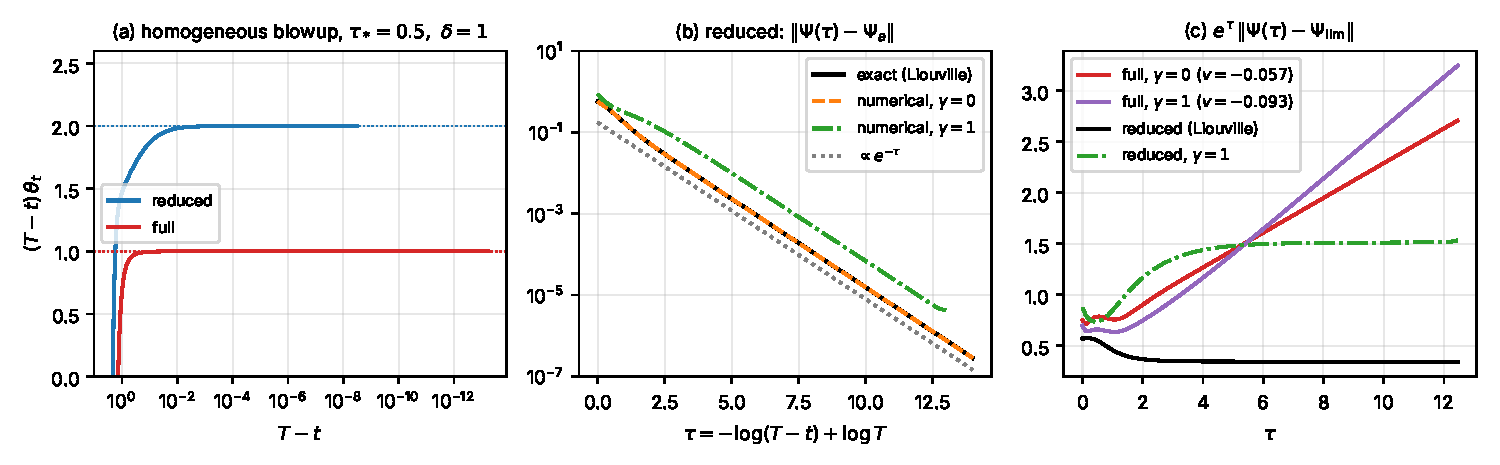
\includegraphics[width=\textwidth]{figures/therm_blowup.pdf}
\caption{(a) Homogeneous blowup of \cref{therm:eq:full,therm:eq:reduced} with
$\varepsilon=0$, $\tau_*=0.5$, $\delta=1$, $\theta(0)=\theta'(0)=0$: $(T-t)\theta_t\to2$ for the reduced and $\to1$
for the full model.  (b) Reduced model, $d=1$: distance to the boosted profile in similarity
variables, exact Liouville solution vs.\ numerics ($\gamma=0$), and the damped case
$\gamma=1$; all decay like $e^{-\tau}$ (gap $1$, sharp).  (c) $e^{\tau}\times$distance to the
limiting profile: constant for the reduced model ($\gamma=0,1$), linear growth ($\tau e^{-\tau}$
decay, Jordan block at $\lambda=-1$) for the full model \cref{therm:eq:fullN}
($\gamma=0,1$; $v$ = fitted tilt).  Code: \texttt{code/therm\_sim1d.py}.}
\label{therm:fig:blowup}
\end{figure}

% ---------------------------------------------------------------------------
\subsection{Arrhenius kinetics: no blowup}
\label{therm:sec:arrhenius}

For $\varepsilon>0$, $f_\varepsilon(\theta)=\delta\exp(\theta/(1+\varepsilon\theta))$ on $\theta>-1/\varepsilon$ (absolute temperature
positive) satisfies $0<f_\varepsilon\le\delta e^{1/\varepsilon}$, and $f_\varepsilon$ together with all derivatives
tends to $0$ as $\theta\downarrow-1/\varepsilon$; hence $f_\varepsilon$ extends by $0$ to a $C^\infty$, bounded,
globally Lipschitz function on $\mathbb{R}$ (hyperbolic models have no maximum principle,
so this extension matters).  Then \cref{therm:eq:reduced} is a semilinear wave
equation with globally Lipschitz nonlinearity, and \cref{therm:eq:full} has in
addition the term $\tau_* f_\varepsilon'(\theta)\theta_t$, linear in $\theta_t$ with a bounded (possibly
anti-damping) coefficient.  Standard energy estimates give global smooth
solutions growing at most exponentially: \emph{there is no finite-time blowup}.
Thermal ``explosion'' is a rapid transition to $\theta=O(1/\varepsilon)$ (temperature rise
of order $\Theta_0$; reactant consumption, neglected here, limits it further).  The FK
blowup is an \emph{intermediate asymptotic} regime, valid while $\varepsilon\theta\ll1$: in
similarity time up to $\tau_{\max}\approx1/(2\varepsilon)$ (reduced) or $\tau_{\max}\approx1/\varepsilon$ (full).  For
typical activation energies $E/(R\Theta_0)=1/\varepsilon\approx20$--$40$ this window spans many
$e$-folds, so the convergence rates above are physically meaningful.

% ---------------------------------------------------------------------------
\subsection{Status, literature and caveats}
\label{therm:sec:status}

\begin{table}[t]
\centering
\small
\begin{tabular}{@{}p{0.31\textwidth}p{0.33\textwidth}p{0.29\textwidth}@{}}
\toprule
Known & Derived here (proof sketch) & Numerical / conjectural\\
\midrule
Liouville's formula \cite{Liouville1853}; MCV law and both model forms
\cite{Cattaneo1958,MendezFortFarjas1999}; for $\square u=e^u$: blowup on a
surface with logarithmic behaviour for data near constants, any $d$
\cite{Kichenassamy1996}; $1$D blowup curves and rates
\cite{Godin2000,Godin2001,AzaiezMasmoudiZaag2016}; Donninger machinery for powers
\cite{DonningerSchoerkhuber2012,DonningerSchoerkhuber2014,DonningerSchoerkhuber2017,Ostermann2024}.
&
Spectra \cref{therm:eq:eigs,therm:eq:eigsfull} with all integer/log cases;
semisimplicity; Jordan block (full); free rates; \cref{therm:thm:reduced}
and \cref{therm:rem:damping}; exact $1$D structure
(\cref{therm:prop:liouville,therm:cor:liouville}); homogeneous dynamics of the full
model; tilted family; \cref{therm:thm:full} (less checked); Arrhenius global existence.
&
$1$D simulations of both models (rates, tilt $=$ slope); exact essential
growth bound $\frac{d+1}2-k$ for the full model; non-ODE (non-homogeneous)
self-similar profiles were not searched for.\\
\bottomrule
\end{tabular}
\caption{Status of the results of \cref{therm:sec}.}
\label{therm:tab:status}
\end{table}

\paragraph{Novelty.}  For the method in general see the survey \cite{Donninger2024}.
We did not find a Donninger-type (similarity variables,
$H^k$, spectral) stability theorem for $u_{tt}-\Delta u=e^u$, nor any analysis of the
MCV-consistent equation with the $\partial_t(e^u)$ nonlinearity.  However,
Kichenassamy's result \cite{Kichenassamy1996} (Fuchsian reduction and Nash--Moser,
data near constants, i.e.\ near the ODE blowup) already implies stability of the
ODE blowup for $\square u=e^u$ in a high-regularity sense, including the
logarithmic terms (absent iff the blowup surface has vanishing scalar
curvature); we have only seen the abstract of \cite{Kichenassamy1996}.
\Cref{therm:thm:reduced} should therefore be viewed as a routine but
quantitative adaptation ($H^k$, $k>d/2$, explicit rate $(T-t)^\omega$, data only on a
ball), while the full Cattaneo model (\cref{therm:sec:full}) appears to be new.
The literature search was limited (search budget), so this assessment is
provisional.

\paragraph{Caveats.}  (1) \Cref{therm:thm:reduced,therm:thm:full} are proof
sketches; the uniform semigroup bounds on the stable subspace (beyond the
quasi-compactness of \cref{therm:lem:free}) and the modulation in $(T,a)$ are
adapted from the power case without writing out all details.
(2) For the full model only the crude essential bound $\frac d2+1-k$ is proved.
(3) Damping requires $\gamma T$ small, reached by Cauchy stability.  (4) The
analysis is local in a light cone; boundary conditions, the Gelfand threshold
$\delta_{\rm crit}$ of bounded domains, and whether blowup occurs at all for given
data are not addressed.  (5) Results concern the FK limit $\varepsilon=0$;
with Arrhenius kinetics there is no blowup (\cref{therm:sec:arrhenius}).
